\documentclass{beamer}
\usetheme{metropolis}
\usepackage{listings}
\usepackage{graphicx}
\usepackage{standalone}
\usepackage{tikz}
\usepackage{tabu}
\usepackage{tikz}
\usepackage{verbatim}
\usepackage{tcolorbox}
\usepackage{appendixnumberbeamer}
\usepackage{booktabs}
\usepackage[scale=2]{ccicons}
\usepackage{pgfplots}
\usepackage{xspace}
\usepgfplotslibrary{dateplot}
\usetikzlibrary{shapes,snakes}

\setbeamertemplate{frame footer}{\insertsection\ // \insertsubsection}

\title{Security Managment of ECM Applications}
\subtitle{Fachpraktikum Information Systems}
\author{Christoph Kleine, Tim Zwietasch, Constantin Weißer}
\date{\today}

\begin{document}

\frame{\titlepage}

\section{Introduction}
\subsection{Idea}
\begin{frame}
	\frametitle{Motivation}
	\begin{tcolorbox}[title=Overall Goal]
		Create an ECM portal for companies that do not want to host
		their data with one of the big providers. The focus is on
		usability and user-friendliness while maintaining security.
	\end{tcolorbox}

	\begin{itemize}
		\item Many companies prefer domestic small solutions
		\item Keep advantages of cloud solutions
		\item IBM's commercial portal as a model
	\end{itemize}
\end{frame}

\begin{frame}
	\frametitle{Motivation}
	\begin{tcolorbox}[title=Our Goal]
		Develop the user, groups and role management for this ECM portal
		based on open-source software.
	\end{tcolorbox}
	\begin{itemize}
		\item Easily extensible web application
		\item Usability
		\item Free and Open-Source Software (FOSS)
	\end{itemize}
\end{frame}

\subsection{FOSS}
\begin{frame}
	\frametitle{Open Source Software}
	\begin{tcolorbox}[title=Why use FOSS components?]
		\begin{itemize}
			\item no licensing costs
			\item scalability!
			\item high security standards
			\item adaptivity
		\end{itemize}
	\end{tcolorbox}
\end{frame}

\section{Security Model}
\subsection{Structure}
\begin{frame}
	\frametitle{Security Model}
	%TODO: class diagram
\end{frame}

\section{Architecture}
\subsection{Overview}
\begin{frame}<1,2>[label=archgraph]
	\only<1,2>{%
		\frametitle{Architecture — Overview}
	}
	\only<3>{%
		\frametitle{Architecture — LDAP-Server}
	}
	\only<4>{%
		\frametitle{Architecture — Java middle layer}
	}
	\only<5>{%
		\frametitle{Architecture — Web-Application}
	}
	\begin{columns}[T]
		\begin{column}{0.48\textwidth}
			\begin{tikzpicture}
				\tikzset{every rectangle node/.style={draw, rectangle, color=gray}}
				\only<5>{%
					\tikzset{every rectangle node/.style={draw, rectangle, color=red}}
				}
				\node (frontend) at (0, 3) {Web-Application};
				\tikzset{every rectangle node/.style={draw, rectangle, color=gray}}
				\only<4>{%
					\tikzset{every rectangle node/.style={draw, rectangle, color=red}}
				}
				\node (middleend) at (0, 0) {Java middle layer};
				\tikzset{every rectangle node/.style={draw, rectangle, color=gray}}
				\only<3>{%
					\tikzset{every rectangle node/.style={draw, rectangle, color=red}}
				}
				\node (ldap) at (0, -3) {LDAP Server};

				\draw[<->] (frontend) to[] (middleend);
				\draw[<->] (middleend) to[] (ldap);
			\end{tikzpicture}
		\end{column}
		\begin{column}{0.48\textwidth}
			\only<2>{%
				\begin{itemize}
					\item Web-Application as user interface
					\item Java middle layer as intermediate program logic
					\item LDAP-Server as persistent storage
				\end{itemize}
			}
			\only<3>{%
				\begin{itemize}
					\item LDAP = ``Lightweight Directory Access Protocol''
					\item persistence back-end (database)
					\item authentication, querying and modification of data
					\item data: users, groups, roles
					\item roles are special groups
				\end{itemize}
			}
			\only<4>{%
				\begin{itemize}
					\item connects front- with back-end
					\item REST interface
					\item connects with LDAP-Server
					\item accepts requests, executes, provides response
					\item stateless
				\end{itemize}
			}
			\only<5>{%
				\begin{itemize}
					\item based on Angular 2
					\item Makes REST calls to middle layer
					\item displays data, responses, handles user interaction
					\item attempt: minimize data transfer
				\end{itemize}
			}
		\end{column}
	\end{columns}
\end{frame}

\subsection{LDAP-Server}
\againframe<3>{archgraph}

\begin{frame}[fragile]
	\frametitle{LDAP Server Structure}
	\lstset{%
		basicstyle=\tiny
	}
	\begin{lstlisting}
SCCM: {
	bindusr : [],
	customer: {
		groups: {
			...
		},
	}
	users: {
		caseadmin: [
			cn: caseadmin,
			objectclass: inetOrgPerson,
			objectclass: organizationalPerson,
			objectclass: person,
			objectclass: top,
			sn: caseadmin,
			displayname: "Case Administrator",
			uid: caseadmin,
			userpassword: ***,
			...
		],
		domainadmin: [...],
		...
	}
}
	\end{lstlisting}
\end{frame}

\subsection{Middle Layer}
\againframe<4>{archgraph}

\begin{frame}
	\frametitle{Middle Layer}
	\begin{itemize}
		\item written in Java
		\item Uses Jersey to provide REST interface
		\item shallow model of data
			\begin{itemize}
				\item User
				\item Group
				\item Role
			\end{itemize}
		\item Actions to manipulate data and query data
		\item \dots\ are passed through to back-end using LDAP requests
		\item \textbf{Authentication}: protects back-end from
			unauthorized access
	\end{itemize}
\end{frame}

\begin{frame}
	\frametitle{Example Request}
	%TODO: nach java middlekack: "Beispiel Request"
\end{frame}

\subsection{Frontend}
\againframe<5>{archgraph}

\begin{frame}
	\frametitle{Angular 2}
\end{frame}

\section{Implementation}

\section{Questions?}

\end{document}
